\section{Theorie}
\label{sec:Theorie}

\cite{sample}

Wirken sogenannte Oberflächenkräfte auf einen festen Körper,
erfahren sie Gestalts- oder Volumenänderungen. Die Spannung
die dabei auftritt hat eine senkrecht zur Oberfläche stehende Komponente, welche
Normalspannung $\sigma$ oder auch Druck $P$ genannt wird, und
eine Tangential-Komponente, welche Schubspannung $\tau$ heißt.
Nimmt der Körper nach der Verformung seine ursprüngliche Gestalt an, spricht
man von einer elastischen Deformation. 

Mit Hilfe des Hookeschen Gesetzes

\begin{equation}
  P = Q \frac{\Delta V}{V} ,
\end{equation}


wird der Zusammenhang  der Spannung und Deformation beschrieben.
Dieses gilt nur für kleine Spannungen. 
Ein Körper besteht aus einem Kristallgitter, also einer regelmäßigen Anordnung von Atomen und Molekülen.
Ist die Symmetrie des Kristalls niedrig, sind die elektrostatischen Kräfte richtungsabhängig, und man braucht insgesamt 36 elastische Konstanten.
Da sich in diesem Experiment aber auf isotrope Körper beschränkt wird, die Konstanten also richtunsunabhängig sind, werden nur 4 Konstanten gebraucht.
Diese sind das Schubmodul $G$, welche die Gestaltelastizität beschreibt,
da Kompressionsmodul $G$, welche die Volumenelastizität beschriebt, das Elastizitätsmodul $E$, zur 
Beschreibung der Längenänderung, wenn eine Normalspannung wirkt, und die Poissonsche Querkontraktionszahl $\mu$, zur Beschreibung der 
Längenänderung senkrecht zur Richtung der Normalspannung.
Die Querkontraktionszahl bestimmt sich aus

\begin{equation}
  \mu = - \frac{\Delta B}{B}\cdot \frac{L}{\Delta L} ,
\end{equation}

mit Breite $B$ und Länge $L$ eines Stabes aus Abbildung (1).
Insgesamt gelten folgende Beziehungen zwischen den Konstanten:

\begin{equation}
  E = 2G(\mu + 1) 
\end{equation}

und

\begin{equation}
  E = 3 (1-2\mu)Q .
\end{equation}

Nur die Konstanten $E$ und $G$ lassen sich experimentell bestimmen; die beiden anderen Konstanten 
müssen aus den obigen Gleichungen berechnet werden. 

\begin{figure}[H]
 \centering
  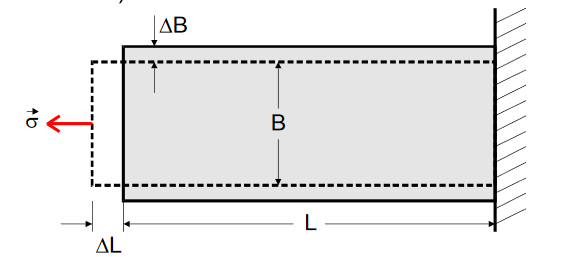
\includegraphics[height=6cm]{Screenshot (7).png}
  \caption{Skizze eines Stabes.}
  \label{fig:drill}
\end{figure}


\subsection{Bestimmung der elastischen Konstanten $G$}

In diesem Versuch werden dynamische Messverfahren beschrieben, in denen die Spannung von der zeit abhängt.
Damit werden Fehler vermieden, die durch elastische Nachwirkung entstehen können. Bei jener stellt sich die Deformation nicht direkt auf einen endgültigen Wert ein.

Um das Schubmodul $G$ zu bestimmen, wird das Prinzip der Torsion angewandt(s. Abbildung (2))
Dabei wird ein Körper an einem Ende fest eingespannt, und am anderen Ende werden an zwei Punkten Kräfte angreifen.
Ein Drehmoment entsteht, welches allerdings auch vom Hebelarm abhängt(dem Abstand des Massepunktes von der Drehachse).
Da dieser nicht konstant ist, muss der Körper in mehrere Hohlzylinder zerlegt werden, und zuletzt über den gesamten Radius integriert werden, was  schließlich auf

\begin{equation}
  M = \frac{2}{\pi}G\frac{R^{4}}{L}\phi
\end{equation}

führt. Es lässt sich eine lineare Beziehung zwischen Drehmoment und Drehwinkel erkennen.
Die Konstante 

\begin{equation}
  D = \frac{\pi G R^{4}}{2L}
\end{equation}
nennt man Richtgröße.

Um die dynamische Variante zu nutzen, wird an das untere Ende des Drahtes ein Körper mit einem bestimmten Trägheitsmoment $\theta$
eingehangen. Tordiert man den Draht nun, wird das System ausgelenkt, und es führt Drehschwingungen aus.
Diese kommt dadurch zustande, dass nun zwei Drehmomente wirken, einmal das in Gleichung (5) beschriebene, und jenes der rotierenden Masse.
Dieses wird beschrieben durch
\begin{equation}
  M_T = \theta \frac{d^{2}\phi}{dt^{2}} .
\end{equation}

Somit lässt sich die Bewegungsgleichung des Systems beschrieben mit

\begin{equation}
  D\phi + \theta \frac{d^{2}\phi}{dt^{2}} = 0 .
\end{equation}

Der Ansatz

\begin{equation}
  \phi(t) = \phi_0 cos \frac{2\pi}{T}t ,
\end{equation}

löst die Gleichung, wobei

\begin{equation}
  T = 2 \pi \sqrt{\theta/D}  
\end{equation}
ist.

Das Trägheitsmoment einer Kugel muss also bekannt sein, und errechnet sich aus

\begin{equation}
  \theta_\text{Kugel} = \frac{2}{5}m_K R_K^{2} .
\end{equation}

Aus den Gleichungen (6), (10) und (11) ergibt sich nun schließlich:

\begin{equation}
 G = \frac{16}{5}\pi \frac{m_K R_K^{2}L}{T^{2}R^{4}} .
\end{equation}

\begin{figure}[H]
 \centering
  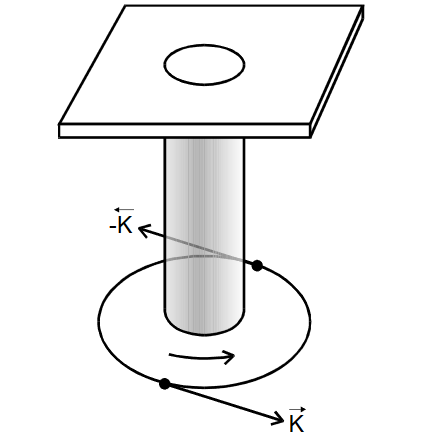
\includegraphics[height=8cm]{Screenshot (9).png}
  \caption{Torsion eines Zylinders.}
  \label{fig:drill}
\end{figure}


\subsection{Bestimmung des magnetischen Moments eines Permanentmagneten}
Das magnetische Moment ist gegeben durch
\begin{equation}
  \vec{m} = p \vec{a} ,
\end{equation}
wobei der Vektor $\vec{a}$ vom Nordpol zum Südpol zeigt, und $p$ die Polstärke ist.
In einem homogenen Magnetfeld $\vec{B}$ wirken auf den Magneten zwei entgegengesetzt gleiche Kräfte. Somit wirkt nur ein Drehmoment $\vec{M}_\text{Mag}$
auf den Magneten

\begin{equation}
  \vec{M}_\text{Mag} = p \vec{a} \times \vec{B} = \vec{m} \times \vec{B} ,
\end{equation}

mit Betrag

\begin{equation}
 M_\text{Mag} = m B sin\gamma
\end{equation}

Wird ein System, welches sich in einem Magnetfeld befindet, ausgelenkt, ergibt sich folgende Bewegungsgleichung:

\begin{equation}
  m B sin\phi + D \phi + \theta \frac{d^{2}\phi}{dt^{2}} = 0 .
\end{equation}

Wieder lässt sich die Gleichung mit einem Kosinus-Ansatz lösen, mit

\begin{equation}
  T_m = 2\pi \sqrt{\frac{\theta}{m B + D}}
\end{equation}
als Periode.



